\documentclass[./../main_file.tex]{subfiles}
\begin{document}
	\subsection{Tổng quan}
	Đây là một mô tả logic về kiến trúc của hệ thống. Mô tả những lớp quan trọng và cách tổ chức những gói dịch vụ và hệ thống con, và cách tổ chức những hệ thống con này vào các lớp. Trong phần này cũng mô tả những ca sử dụng quan trọng nhất, ví dụ những khía cạnh linh hoạt của kiến trúc hệ thống. Biểu đồ lớp có thể được đưa vào để minh họa các mối quan hệ giữa kiến trúc quan trọng các lớp, hệ thống con, gói và lớp.
	\begin{figure}[H]
		\centering
		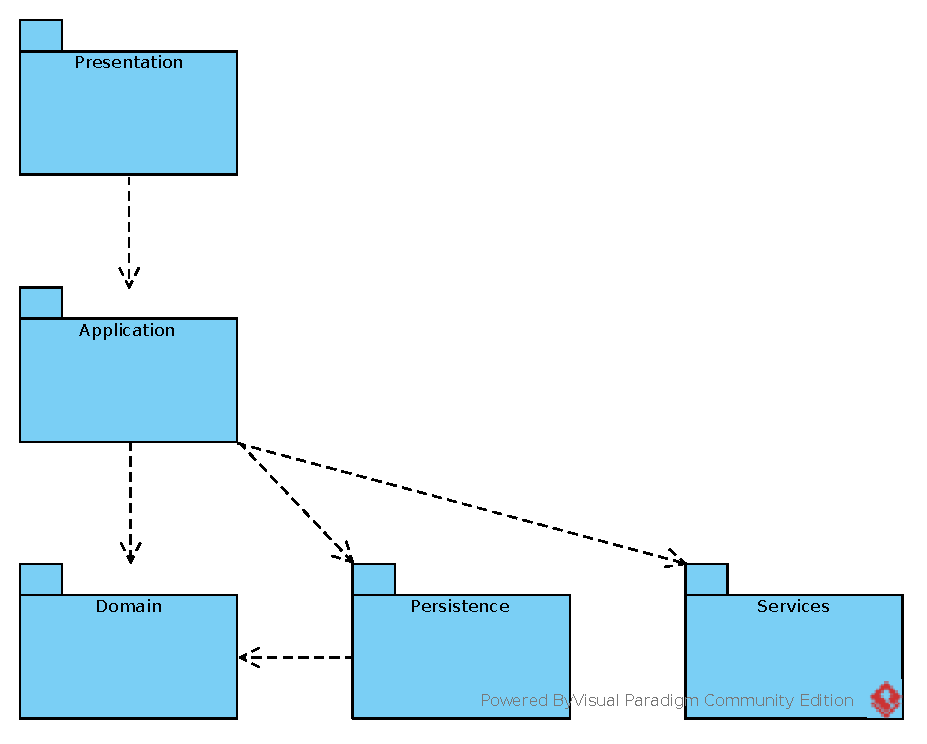
\includegraphics[width=\linewidth]{./images/logic_view_package_diagram.eps}
		\caption{Biểu đồ các gói trong khung nhìn logic}
	\end{figure}
	Khung nhìn logic của Hệ thống giảng dạy và học trực tuyến Moodle Plus bao gồm 5 gói:
	\begin{description}
		\item[Giao diện (Presentation)] chứa các lớp cho mỗi biểu mẫu mà các tác nhân sử dụng để giao tiếp với Hệ thống.
		\item[Ứng dụng (Application)] chứa các lớp xử lý chính cho hệ thống.
		\item[Miền (Domain)] chứa các gói chứa các lớp để hỗ trợ về người dùng, khóa học, xã hội.
		\item[Nhất quán (Persistence)] chứa các lớp để đảm bảo tính nhất quán của dữ liệu.
		\item[Dịch vụ (Services)] chứa các lớp để cung cấp các lớp hệ thống cho mục đích bảo trì.
	\end{description}

	\subsection{Các gói thiết kế kiến trúc quan trọng}
	\subsubsection{Gói miền (Domain Package)}
	\paragraph{Mô tả ngắn gọn}
	Gói này chứa các gói chứa các lớp để hỗ trợ về khóa học, tài khoản, xã hội. Gói miền bao gồm 3 gói con sau đây:
	\begin{description}
		\item[Gói khóa học (course package)] chứa thông tin về khóa học, sinh viên và giảng viên trong khóa học.
		\item[Gói người dùng (user package)] chứa tất cả các lớp xác thực người dùng, thông tin tài khoản và thông tin cá nhân người dùng
		\item[Gói xã hội (social package)] chứa tất cả các phương thức giúp các user có thể giao tiếp được với nhau.
	\end{description}
	\paragraph{Biểu đồ} ~\\
	\begin{figure}[htb]
		\centering
				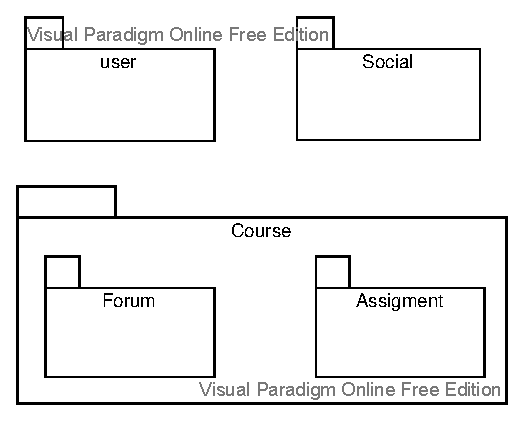
\includegraphics[width=\linewidth]{./images/subpackageindomaindigram.eps}
		\caption{Biểu đồ gói con trong miền}
	\end{figure}

	\paragraph{Gói Course} ~\\'
	\begin{figure}[H]
		\centering
		\resizebox{\textwidth}{!}{\input{./images/domain_package_course.pdf_tex}}
		\caption{Biểu đồ gói con trong miền}
	\end{figure}
		
	\paragraph{Gói User} ~\\
	\begin{figure}[H]
		\centering
		\resizebox{0.9\textwidth}{!}{\input{./images/PackageUser_LogicalView.pdf_tex}}
		\caption{Biểu đồ gói con trong miền}
	\end{figure}

	\paragraph{Gói Social}~\\
	\begin{figure}[H]
		\centering
				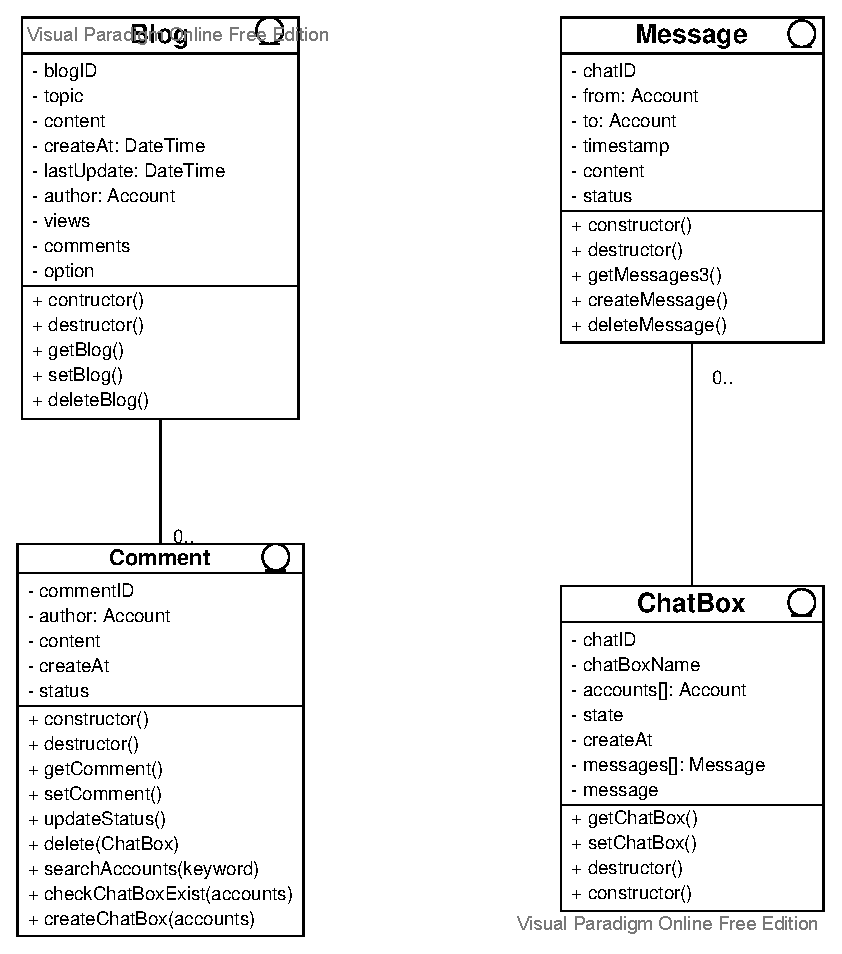
\includegraphics[width=\linewidth]{./images/PackageSocial_LogicalView.eps}
		\caption{Biểu đồ gói con trong miền}
	\end{figure}
	
	\subsubsection{Gói giao diện}
	\paragraph{Mô tả ngắn gọn}
	Gói này bao gồm các lớp với từng form mà tác nhân sử dụng để tương tác với hệ thống. Các lớp biên tồn tại để thực hiện chức năng đăng nhập, đăng ký, quản lý lớp học, nhắn tin, tổ chức lớp học trực tuyến, làm bài kiểm tra, nộp bài tập về nhà và quản lý hệ thống.
	\paragraph{Biểu đồ} ~\\
	\begin{figure}[H]
		\centering
				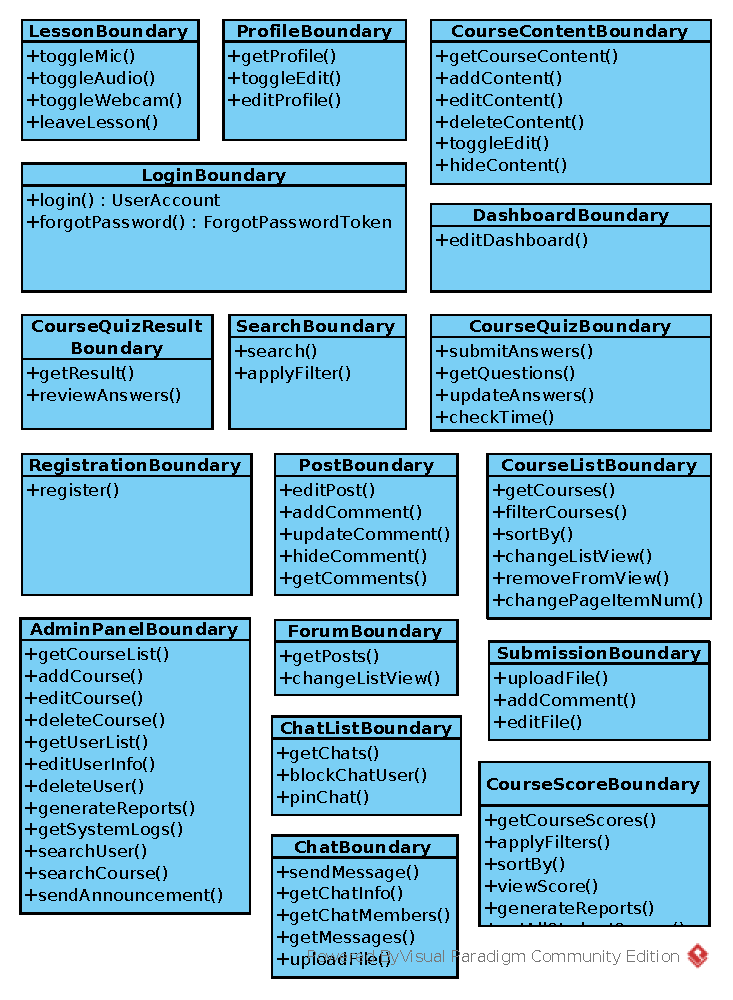
\includegraphics[width=\linewidth]{./images/PresentationPackage.eps}
		\caption{Biểu đồ gói gói giao diện}
	\end{figure}
	\subsubsection{Gói ứng dụng}
	\paragraph{Mô tả ngắn gọn}
	Gói này chứa các lớp cho chức năng xử lý chính trong hệ thống.
	\paragraph{Biểu đồ}~\\
	\begin{figure}[H]
		\centering
		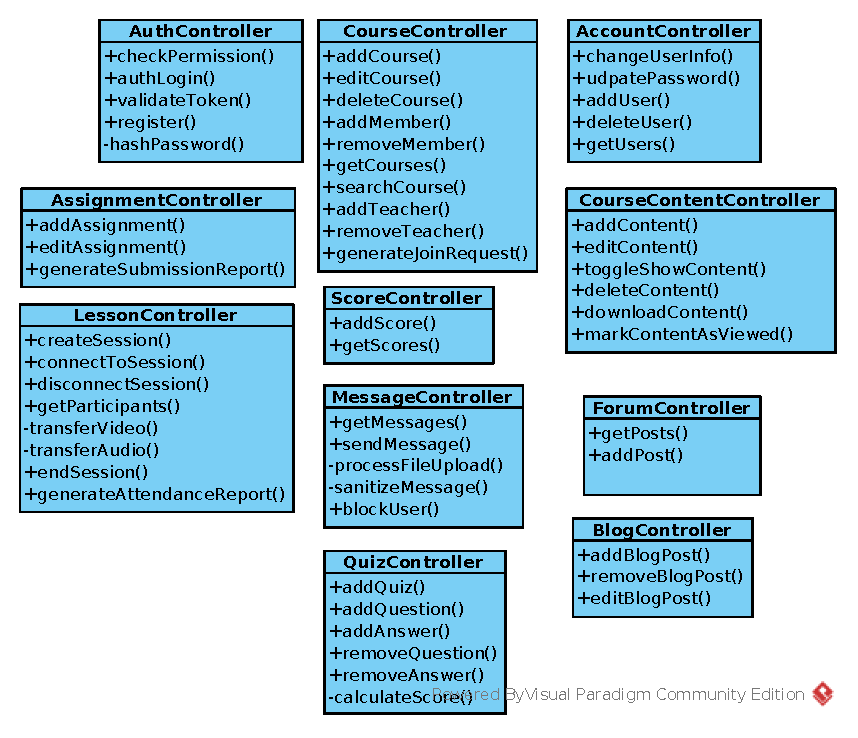
\includegraphics[width=\linewidth]{./images/application_package.eps}
		\caption{Biểu đồ gói gói giao diện}
	\end{figure}
	\subsection{Gói nhất quán}
	\paragraph{Mô tả ngắn gọn}
	Gói này chứa các gói dữ liệu để đảm bảo tính nhất quán của dữ liệu. Bốn toán tử: thêm, sửa, xóa, cập nhật là bốn chức năng chính được thực hiện trong các ứng dụng cơ sở dữ liệu.
	\paragraph{Biểu đồ}~\\
		\begin{figure}[H]
		\centering
				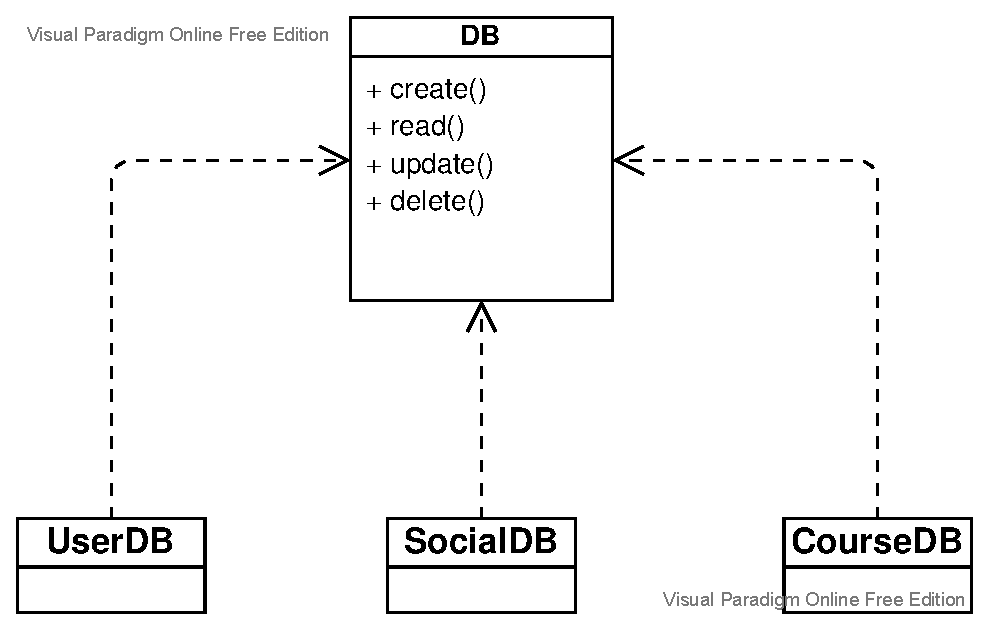
\includegraphics[width=\linewidth]{./images/PackagePersistence_LogicalView.eps}
		\caption{Biểu đồ gói nhất quán}
	\end{figure}
	\subsubsection{Gói dịch vụ}
	Việc bảo trì hiện tại sẽ được thực hiện thủ công. Vì vậy, gói dịch vụ chưa được phát triển.
	
\end{document}